\documentclass[border=10pt]{standalone}
\usepackage{tikz}
\usetikzlibrary{arrows.meta, calc, shadings}

\begin{document}
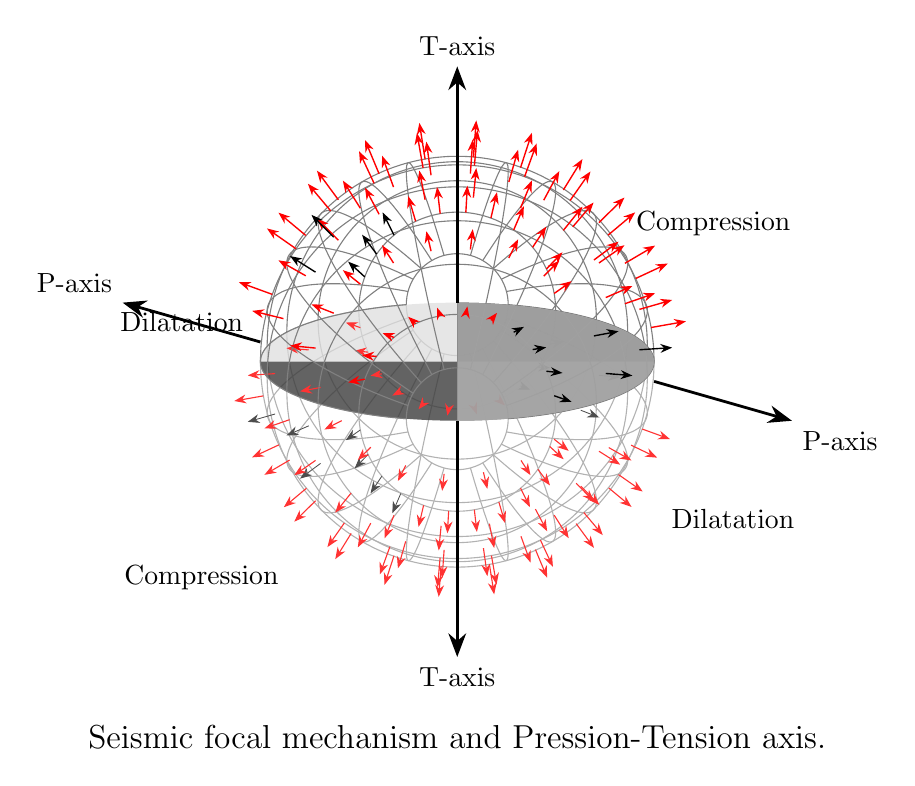
\begin{tikzpicture}[scale=2.5, line join=round]
  
  % Define colors
  \definecolor{darkgray}{RGB}{60,60,60}
  \definecolor{lightgray}{RGB}{220,220,220}
  
  % Draw the sphere mesh - back hemisphere
  \foreach \lat in {-75,-60,...,75} {
    \draw[black!30, thin] plot[domain=-180:0, samples=40, smooth] 
      ({cos(\x)*cos(\lat)}, {sin(\x)*cos(\lat) + 0.3*sin(\lat)});
  }
  \foreach \lon in {-180,-165,...,-15} {
    \draw[black!30, thin] plot[domain=-75:75, samples=30, smooth] 
      ({cos(\lon)*cos(\x)}, {sin(\lon)*cos(\x) + 0.3*sin(\x)});
  }
  
  % Fill quadrants - back
  \fill[lightgray, opacity=0.7] plot[domain=-90:0, samples=30] 
    ({cos(\x)}, {sin(\x)*0.3}) -- 
    plot[domain=0:-90, samples=30] ({-cos(\x)}, {-sin(\x)*0.3}) -- cycle;
  
  \fill[darkgray, opacity=0.8] plot[domain=0:90, samples=30] 
    ({cos(\x)}, {sin(\x)*0.3}) -- 
    plot[domain=90:0, samples=30] ({-cos(\x)}, {-sin(\x)*0.3}) -- cycle;
  
  % Draw dilatation arrows (back side)
  \foreach \angle in {-170,-155,...,-10} {
    \foreach \elev in {-60,-40,-20,0,20,40,60} {
      \pgfmathsetmacro{\x}{cos(\angle)*cos(\elev)}
      \pgfmathsetmacro{\y}{sin(\angle)*cos(\elev) + 0.3*sin(\elev)}
      \pgfmathsetmacro{\condition}{int(sign(sin(\angle + \elev)))}
      \ifnum\condition>0
        \draw[-{Stealth[length=1.5mm]}, black!70, line width=0.3pt] 
          (\x, \y) -- ++({0.15*\x}, {0.15*\y});
      \fi
    }
  }
  
  % Draw compression arrows (back side)
  \foreach \angle in {-170,-155,...,-10} {
    \foreach \elev in {-60,-40,-20,0,20,40,60} {
      \pgfmathsetmacro{\x}{cos(\angle)*cos(\elev)}
      \pgfmathsetmacro{\y}{sin(\angle)*cos(\elev) + 0.3*sin(\elev)}
      \pgfmathsetmacro{\condition}{int(sign(sin(\angle + \elev)))}
      \ifnum\condition<0
        \draw[-{Stealth[length=1.5mm]}, red!80, line width=0.4pt] 
          (\x, \y) -- ++({0.15*\x}, {0.15*\y});
      \fi
    }
  }
  
  % Draw the sphere mesh - front hemisphere
  \foreach \lat in {-75,-60,...,75} {
    \draw[black!50, thin] plot[domain=0:180, samples=40, smooth] 
      ({cos(\x)*cos(\lat)}, {sin(\x)*cos(\lat) + 0.3*sin(\lat)});
  }
  \foreach \lon in {0,15,...,180} {
    \draw[black!50, thin] plot[domain=-75:75, samples=30, smooth] 
      ({cos(\lon)*cos(\x)}, {sin(\lon)*cos(\x) + 0.3*sin(\x)});
  }
  
  % Fill quadrants - front
  \fill[darkgray, opacity=0.85] plot[domain=0:90, samples=30] 
    ({cos(\x)}, {sin(\x)*0.3}) -- 
    plot[domain=90:0, samples=30] ({cos(\x)}, {-sin(\x)*0.3}) -- cycle;
  
  \fill[lightgray, opacity=0.6] plot[domain=-90:0, samples=30] 
    ({cos(\x)}, {sin(\x)*0.3}) -- 
    plot[domain=0:-90, samples=30] ({cos(\x)}, {-sin(\x)*0.3}) -- cycle;
  
  % Draw compression arrows (front side - upper right)
  \foreach \angle in {10,25,...,170} {
    \foreach \elev in {-60,-40,-20,0,20,40,60} {
      \pgfmathsetmacro{\x}{cos(\angle)*cos(\elev)}
      \pgfmathsetmacro{\y}{sin(\angle)*cos(\elev) + 0.3*sin(\elev)}
      \pgfmathsetmacro{\condition}{int(sign(sin(\angle + \elev)))}
      \ifnum\condition>0
        \draw[-{Stealth[length=1.5mm]}, red, line width=0.5pt] 
          (\x, \y) -- ++({0.18*\x}, {0.18*\y});
      \fi
    }
  }
  
  % Draw dilatation arrows (front side - lower right)
  \foreach \angle in {10,25,...,170} {
    \foreach \elev in {-60,-40,-20,0,20,40,60} {
      \pgfmathsetmacro{\x}{cos(\angle)*cos(\elev)}
      \pgfmathsetmacro{\y}{sin(\angle)*cos(\elev) + 0.3*sin(\elev)}
      \pgfmathsetmacro{\condition}{int(sign(sin(\angle + \elev)))}
      \ifnum\condition<0
        \draw[-{Stealth[length=1.5mm]}, black, line width=0.5pt] 
          (\x, \y) -- ++({0.18*\x}, {0.18*\y});
      \fi
    }
  }
  
  % Draw axes
  \draw[-{Stealth[length=3mm]}, line width=1pt] (0, 0.3) -- (0, 1.5) 
    node[above] {T-axis};
  \draw[-{Stealth[length=3mm]}, line width=1pt] (0, -0.3) -- (0, -1.5) 
    node[below] {T-axis};
  \draw[-{Stealth[length=3mm]}, line width=1pt] (-1, 0.1) -- (-1.7, 0.3) 
    node[above left] {P-axis};
  \draw[-{Stealth[length=3mm]}, line width=1pt] (1, -0.1) -- (1.7, -0.3) 
    node[below right] {P-axis};
  
  % Labels
  \node[align=center] at (1.3, 0.7) {Compression};
  \node[align=center] at (-1.4, 0.2) {Dilatation};
  \node[align=center] at (1.4, -0.8) {Dilatation};
  \node[align=center] at (-1.3, -1.1) {Compression};
  
  % Caption
  \node[below, align=center, font=\large] at (0, -1.8) 
    {Seismic focal mechanism and Pression-Tension axis.};
    
\end{tikzpicture}
\end{document}